\documentclass[a4paper,12pt]{report}
% book report(no part) article(no part/section) letter slides
%      ------          -------
% chapter c section c subsection c subsubsection c paragraph c subparagraph

% ----------------------------------
% PACKAGES
% ----------------------------------

% \usepackage[noTeX]{mmap}
\usepackage{cmap}
\usepackage[T1,T2A]{fontenc}
\usepackage[utf8]{inputenc}
% \usepackage{hyphsubst}
\usepackage[english,russian]{babel}
\usepackage[left=1in,right=1in,top=1in,bottom=1in,paper=a4paper]{geometry}
\usepackage{amsmath,amsfonts,amsthm,amssymb,mathtools}
\usepackage{lipsum}
% \usepackage{extsizes} -- conflict with geometry package
\usepackage{xfrac}
\usepackage{enumitem}
\usepackage{bookmark}

% ----------------------------------
% custom packages
% \usepackage{bigints}
% ----------------------------------

\usepackage{hyperref,theoremref}
\usepackage{cleveref}
\usepackage{nameref}
\hypersetup{
    colorlinks=true,
    linkcolor=blue,
    filecolor=magenta,
    urlcolor=blue,
    pdftitle={assignment},
}
\urlstyle{same}
\newcommand\myref[1]{\hyperref[#1]{#1}}

\usepackage{etoolbox}
\usepackage{multicol,array}
\usepackage{pdfpages}

\usepackage{graphicx}
\graphicspath{ {./graphics/} }

\mathtoolsset{showonlyrefs=false}
% \usepackage{leqno}

\usepackage{biblatex}
% \usepackage{cite}
\usepackage{csquotes}
% \renewcommand{\refname}{Список источников}  % default: "Список литературы" (article)
% \renewcommand{\bibname}{Список литературы} % default: "Литература" (book и report)


% ----------------------------------
% COMMANDS
% ----------------------------------

% bigcdot ( \cdot < \bigcdot < \bullet )
\makeatletter
\newcommand*\bigcdot{\mathpalette\bigcdot@{.5}}
\newcommand*\bigcdot@[2]{\mathbin{\vcenter{\hbox{\scalebox{#2}{$\m@th#1\bullet$}}}}}
\makeatother

% deliminator
\DeclarePairedDelimiter{\abs}{\lvert}{\rvert}
\DeclarePairedDelimiter{\norm}{\lVert}{\rVert}
\DeclarePairedDelimiter{\ceil}{\lceil}{\rceil}
\DeclarePairedDelimiter{\floor}{\lfloor}{\rfloor}
\DeclarePairedDelimiter{\round}{\lfloor}{\rceil}

\usepackage[dvipsnames, table, xcdraw]{xcolor} % load before pgfplots
\usepackage{pgfplots}
\pgfplotsset{compat=1.18}
\usepackage{tikz}
\usetikzlibrary{positioning}
\usetikzlibrary{arrows.meta}
\usetikzlibrary{decorations.pathreplacing,calligraphy}
\usetikzlibrary{shapes.geometric}
\usepgfplotslibrary{colorbrewer}
\usepackage[export]{adjustbox}
\usepackage{subfig}

% ----------------------------------
% range [a,b]
% ----------------------------------
\newcommand\abseg{\ensuremath{[a,b]}}
\newcommand\abint{\ensuremath{(a,b)}}

% ----------------------------------
% bigcdot ( \cdot < \bigcdot < \bullet )
% ----------------------------------
\makeatletter
\newcommand*\bigcdot{\mathpalette\bigcdot@{.5}}
\newcommand*\bigcdot@[2]{\mathbin{\vcenter{\hbox{\scalebox{#2}{$\m@th#1\bullet$}}}}}
\makeatother

% ----------------------------------
% argmax, argmin
% ----------------------------------
\DeclareMathOperator*{\argmax}{argmax}
\DeclareMathOperator*{\argmin}{argmin}

% ----------------------------------
% deliminator
% ----------------------------------
\DeclarePairedDelimiter{\abs}{\lvert}{\rvert}
\DeclarePairedDelimiter{\norm}{\lVert}{\rVert}
\DeclarePairedDelimiter{\ceil}{\lceil}{\rceil}
\DeclarePairedDelimiter{\floor}{\lfloor}{\rfloor}
\DeclarePairedDelimiter{\round}{\lfloor}{\rceil}

% \DeclareMathOperator{\Ext}{Ext} % Ext functor
% \DeclareMathOperator{\Tor}{Tor} % Tor functor
\DeclareMathOperator{\sgn}{sgn}
% \newcommand{\gl}{\opname{\mathfrak{gl}}} % frak gl group
% \renewcommand{\sl}{\opname{\mathfrak{sl}}} % frak sl group chktex 6

% Number sets
\newcommand{\RR}{\ensuremath{\mathbb{R}}}
\newcommand{\NN}{\ensuremath{\mathbb{N}}}
\newcommand{\ZZ}{\ensuremath{\mathbb{Z}}}
\newcommand{\QQ}{\ensuremath{\mathbb{Q}}}
\newcommand{\CC}{\ensuremath{\mathbb{C}}}
\newcommand{\PP}{\ensuremath{\mathbb{P}}}
\newcommand{\HH}{\ensuremath{\mathbb{H}}}
\newcommand{\FF}{\ensuremath{\mathbb{F}}}
\newcommand{\EE}{\ensuremath{\mathbb{E}}}

\DeclareMathOperator{\GL}{GL} % General linear group
\DeclareMathOperator{\SL}{SL} % Special linear group



% ---------------------------------------
% Math Black Board (bb):
% ---------------------------------------
% Capital Letters
\newcommand{\bbA}{\mathbb{A}}	\newcommand{\bbB}{\mathbb{B}}
\newcommand{\bbC}{\mathbb{C}}	\newcommand{\bbD}{\mathbb{D}}
\newcommand{\bbE}{\mathbb{E}}	\newcommand{\bbF}{\mathbb{F}}
\newcommand{\bbG}{\mathbb{G}}	\newcommand{\bbH}{\mathbb{H}}
\newcommand{\bbI}{\mathbb{I}}	\newcommand{\bbJ}{\mathbb{J}}
\newcommand{\bbK}{\mathbb{K}}	\newcommand{\bbL}{\mathbb{L}}
\newcommand{\bbM}{\mathbb{M}}	\newcommand{\bbN}{\mathbb{N}}
\newcommand{\bbO}{\mathbb{O}}	\newcommand{\bbP}{\mathbb{P}}
\newcommand{\bbQ}{\mathbb{Q}}	\newcommand{\bbR}{\mathbb{R}}
\newcommand{\bbS}{\mathbb{S}}	\newcommand{\bbT}{\mathbb{T}}
\newcommand{\bbU}{\mathbb{U}}	\newcommand{\bbV}{\mathbb{V}}
\newcommand{\bbW}{\mathbb{W}}	\newcommand{\bbX}{\mathbb{X}}
\newcommand{\bbY}{\mathbb{Y}}	\newcommand{\bbZ}{\mathbb{Z}}



% ---------------------------------------
% Math Cal (cal):
% ---------------------------------------
% Capital Letters
\newcommand{\calA}{\mathcal{A}}	\newcommand{\calB}{\mathcal{B}}
\newcommand{\calC}{\mathcal{C}}	\newcommand{\calD}{\mathcal{D}}
\newcommand{\calE}{\mathcal{E}}	\newcommand{\calF}{\mathcal{F}}
\newcommand{\calG}{\mathcal{G}}	\newcommand{\calH}{\mathcal{H}}
\newcommand{\calI}{\mathcal{I}}	\newcommand{\calJ}{\mathcal{J}}
\newcommand{\calK}{\mathcal{K}}	\newcommand{\calL}{\mathcal{L}}
\newcommand{\calM}{\mathcal{M}}	\newcommand{\calN}{\mathcal{N}}
\newcommand{\calO}{\mathcal{O}}	\newcommand{\calP}{\mathcal{P}}
\newcommand{\calQ}{\mathcal{Q}}	\newcommand{\calR}{\mathcal{R}}
\newcommand{\calS}{\mathcal{S}}	\newcommand{\calT}{\mathcal{T}}
\newcommand{\calU}{\mathcal{U}}	\newcommand{\calV}{\mathcal{V}}
\newcommand{\calW}{\mathcal{W}}	\newcommand{\calX}{\mathcal{X}}
\newcommand{\calY}{\mathcal{Y}}	\newcommand{\calZ}{\mathcal{Z}}



% ---------------------------------------
% Math Bold (bld) Font:
% ---------------------------------------
% Capital Letters
\newcommand{\bldA}{\boldsymbol{A}}	\newcommand{\bldB}{\boldsymbol{B}}
\newcommand{\bldC}{\boldsymbol{C}}	\newcommand{\bldD}{\boldsymbol{D}}
\newcommand{\bldE}{\boldsymbol{E}}	\newcommand{\bldF}{\boldsymbol{F}}
\newcommand{\bldG}{\boldsymbol{G}}	\newcommand{\bldH}{\boldsymbol{H}}
\newcommand{\bldI}{\boldsymbol{I}}	\newcommand{\bldJ}{\boldsymbol{J}}
\newcommand{\bldK}{\boldsymbol{K}}	\newcommand{\bldL}{\boldsymbol{L}}
\newcommand{\bldM}{\boldsymbol{M}}	\newcommand{\bldN}{\boldsymbol{N}}
\newcommand{\bldO}{\boldsymbol{O}}	\newcommand{\bldP}{\boldsymbol{P}}
\newcommand{\bldQ}{\boldsymbol{Q}}	\newcommand{\bldR}{\boldsymbol{R}}
\newcommand{\bldS}{\boldsymbol{S}}	\newcommand{\bldT}{\boldsymbol{T}}
\newcommand{\bldU}{\boldsymbol{U}}	\newcommand{\bldV}{\boldsymbol{V}}
\newcommand{\bldW}{\boldsymbol{W}}	\newcommand{\bldX}{\boldsymbol{X}}
\newcommand{\bldY}{\boldsymbol{Y}}	\newcommand{\bldZ}{\boldsymbol{Z}}
% Small Letters
\newcommand{\blda}{\boldsymbol{a}}	\newcommand{\bldb}{\boldsymbol{b}}
\newcommand{\bldc}{\boldsymbol{c}}	\newcommand{\bldd}{\boldsymbol{d}}
\newcommand{\blde}{\boldsymbol{e}}	\newcommand{\bldf}{\boldsymbol{f}}
\newcommand{\bldg}{\boldsymbol{g}}	\newcommand{\bldh}{\boldsymbol{h}}
\newcommand{\bldi}{\boldsymbol{i}}	\newcommand{\bldj}{\boldsymbol{j}}
\newcommand{\bldk}{\boldsymbol{k}}	\newcommand{\bldl}{\boldsymbol{l}}
\newcommand{\bldm}{\boldsymbol{m}}	\newcommand{\bldn}{\boldsymbol{n}}
\newcommand{\bldo}{\boldsymbol{o}}	\newcommand{\bldp}{\boldsymbol{p}}
\newcommand{\bldq}{\boldsymbol{q}}	\newcommand{\bldr}{\boldsymbol{r}}
\newcommand{\blds}{\boldsymbol{s}}	\newcommand{\bldt}{\boldsymbol{t}}
\newcommand{\bldu}{\boldsymbol{u}}	\newcommand{\bldv}{\boldsymbol{v}}
\newcommand{\bldw}{\boldsymbol{w}}	\newcommand{\bldx}{\boldsymbol{x}}
\newcommand{\bldy}{\boldsymbol{y}}	\newcommand{\bldz}{\boldsymbol{z}}



% ---------------------------------------
% Math Script (src) Font:
% ---------------------------------------
\newcommand{\srcA}{{\mathscr{A}}}   \newcommand{\srcB}{{\mathscr{B}}}
\newcommand{\srcC}{{\mathscr{C}}}   \newcommand{\srcD}{{\mathscr{D}}}
\newcommand{\srcE}{{\mathscr{E}}}   \newcommand{\srcF}{{\mathscr{F}}}
\newcommand{\srcG}{{\mathscr{G}}}   \newcommand{\srcH}{{\mathscr{H}}}
\newcommand{\srcI}{{\mathscr{I}}}   \newcommand{\srcJ}{{\mathscr{J}}}
\newcommand{\srcK}{{\mathscr{K}}}   \newcommand{\srcL}{{\mathscr{L}}}
\newcommand{\srcM}{{\mathscr{M}}}   \newcommand{\srcN}{{\mathscr{N}}}
\newcommand{\srcO}{{\mathscr{O}}}   \newcommand{\srcP}{{\mathscr{P}}}
\newcommand{\srcQ}{{\mathscr{Q}}}   \newcommand{\srcR}{{\mathscr{R}}}
\newcommand{\srcS}{{\mathscr{S}}}   \newcommand{\srcT}{{\mathscr{T}}}
\newcommand{\srcU}{{\mathscr{U}}}   \newcommand{\srcV}{{\mathscr{V}}}
\newcommand{\srcW}{{\mathscr{W}}}   \newcommand{\srcX}{{\mathscr{X}}}
\newcommand{\srcY}{{\mathscr{Y}}}   \newcommand{\srcZ}{{\mathscr{Z}}}



% ---------------------------------------
% Math Fraktur (frk) Font:
% --------------------------------------
% Capital Letters
\newcommand{\frkA}{\mathfrak{A}}	\newcommand{\frkB}{\mathfrak{B}}
\newcommand{\frkC}{\mathfrak{C}}	\newcommand{\frkD}{\mathfrak{D}}
\newcommand{\frkE}{\mathfrak{E}}	\newcommand{\frkF}{\mathfrak{F}}
\newcommand{\frkG}{\mathfrak{G}}	\newcommand{\frkH}{\mathfrak{H}}
\newcommand{\frkI}{\mathfrak{I}}	\newcommand{\frkJ}{\mathfrak{J}}
\newcommand{\frkK}{\mathfrak{K}}	\newcommand{\frkL}{\mathfrak{L}}
\newcommand{\frkM}{\mathfrak{M}}	\newcommand{\frkN}{\mathfrak{N}}
\newcommand{\frkO}{\mathfrak{O}}	\newcommand{\frkP}{\mathfrak{P}}
\newcommand{\frkQ}{\mathfrak{Q}}	\newcommand{\frkR}{\mathfrak{R}}
\newcommand{\frkS}{\mathfrak{S}}	\newcommand{\frkT}{\mathfrak{T}}
\newcommand{\frkU}{\mathfrak{U}}	\newcommand{\frkV}{\mathfrak{V}}
\newcommand{\frkW}{\mathfrak{W}}	\newcommand{\frkX}{\mathfrak{X}}
\newcommand{\frkY}{\mathfrak{Y}}	\newcommand{\frkZ}{\mathfrak{Z}}
% Small Letters
\newcommand{\frka}{\mathfrak{a}}	\newcommand{\frkb}{\mathfrak{b}}
\newcommand{\frkc}{\mathfrak{c}}	\newcommand{\frkd}{\mathfrak{d}}
\newcommand{\frke}{\mathfrak{e}}	\newcommand{\frkf}{\mathfrak{f}}
\newcommand{\frkg}{\mathfrak{g}}	\newcommand{\frkh}{\mathfrak{h}}
\newcommand{\frki}{\mathfrak{i}}	\newcommand{\frkj}{\mathfrak{j}}
\newcommand{\frkk}{\mathfrak{k}}	\newcommand{\frkl}{\mathfrak{l}}
\newcommand{\frkm}{\mathfrak{m}}	\newcommand{\frkn}{\mathfrak{n}}
\newcommand{\frko}{\mathfrak{o}}	\newcommand{\frkp}{\mathfrak{p}}
\newcommand{\frkq}{\mathfrak{q}}	\newcommand{\frkr}{\mathfrak{r}}
\newcommand{\frks}{\mathfrak{s}}	\newcommand{\frkt}{\mathfrak{t}}
\newcommand{\frku}{\mathfrak{u}}	\newcommand{\frkv}{\mathfrak{v}}
\newcommand{\frkw}{\mathfrak{w}}	\newcommand{\frkx}{\mathfrak{x}}
\newcommand{\frky}{\mathfrak{y}}	\newcommand{\frkz}{\mathfrak{z}}


\title{Отчет по курсовой работе\\"Построение нейронной сети Кохонена"}
\author{КМБО-01-21, Рустем Сиразетдинов}

\begin{document}

    \maketitle
    \newpage
    \tableofcontents
    \pagebreak

\chapter{Предисловие}
В современном мире работа исследователей все чаще направлена на
изучение и развитие \textit{искусственного интеллекта} (далее -
ИИ). Работы в этой области обладают значительным
прикладным потенциалом. Но уже сейчас их применение
крайне разнообразно: предсказание заболеваний на основе анализов человека,
распознавание биометрических данных, обработка больших данных и предсказания на их основе, голосовые
ассистенты, компьютерное зрение и тд.
Особое место занимает генеративный искусственный интеллект,
создающий, например, мультимедийные материалы или тексты,
неотличимые от результатов человеческих усилий.

Все это результаты ученых, пытающихся создать структуры подобные человеческой нервной
системе в цифровом пространстве. Mы, конечно, имеем ввиду
\textit{искусственные нейронные сети} (далее - нейронные сети) - одна из самых
популярных и успешных реализаций ИИ, воссоздающая нервную систему
человека лишь с некоторыми упрощениями. Конечно, здесь невозможно не
упомянуть и огромную работу нейробилогов, предоставляющих
информацию о нервной системе человека, а также все серьезные проблемы
урегулирования развития ИИ, однако оставим их рассмотрение за рамками текущего отчета.

В этой работе мы постараемся дать некоторые начальные положения
устройства и работы нейронных сетей, более подробно рассмотрим саморегулирующиеся сети, что представляют класс
сетей с обучением без подкрепления, приведем реализацию такой
нейронной сети и продемонстрируем ее работу на примере задачи
распознавания цифр.

\chapter{Введение} \label{chapter:Introduction}
\section{Знакомство с нейронными сетями}
Исследования по нейронным сетям связаны с тем, что способ обработки
информации человеческим мозгом в корне отличается от методов,
применяемых обычными цифровыми компьютерами. Мозг представляет собой
сложный, нелинейный, параллельный компьютер. Важная его особенность
заключается в организации своих структурных компонент, называемых
\textit{нейронами}, так, чтобы они могли выполнять конкретные задачи
во много раз быстрее, чем могут позволить самые быстродействующие
современные компьютеры. Примером такой задачи обработки информации
служит обычное \textit{зрение}. В функции зрительной системы входит
создание представления окружающего мира в таком виде, который
обеспечивает возможность взаимодействия с этим миром. Т.е. мозг
последовательно выполняет ряд задач распознавания и на это ему
требуется порядка 100-200 миллисекунд, в то время как выполнение
аналогичных задач даже меньшей сложности на компьютере может занять
несколько дней.

Что позволяет мозгу достичь такого результата? Дело в том, что
при рождении мозг человека крайне \textit{пластичен}, т.е. легко позволяет
нервной системе подстраиваться (настраивать нейроны и синопсисы) под окружающую среду на основе
накапливающегося опыта. Аналогично, в искусственных нейронных сетях
работа проводится искусственными нейронами, которые прошли процесс
\textit{обучения}. Процедура, использующаяся для процесса обучения,
называется \textit{алгоритмом обучения}. Ее задача состоит в
выстраивании в определенном порядке синаптических весов сети для
обеспечения правильных взаимосвязей между самими нейронами. Таким
образом мы пришли к следующему определению искусственной нейронной
сети.

\begin{quote}
    \textbf{Нейронная сеть} - это распределенный параллельный
    процессор, состоящий из элементарных единиц обработки информации,
    накапливающих экспериментальные знания и предоставляющих их для
    последующей обработки.
\end{quote}

\section{Модели нейронов}
\textit{Нейрон} представляет собой единицу обработки информации в
нейронной сети. На рис. \ref{fig:nonlinear neuron model} показана модель нейрона, лежащего в
основе нейронных сетей. В модели можно выделить три основных элемента.

\begin{figure}[!htb]
\centering
\resizebox{0.70\paperwidth}{!}{%
    \begin{tikzpicture}
        \tikzstyle{vertex}=[auto=left,circle,fill=red!25,opacity=.8,
            draw=red,minimum size=20pt,inner sep=0pt]

            \node[vertex] (n0)  at (-4,3) {$\omega_{k0}$};
            \node[left = 1.5cm of n0] (x0) at (n0) {$x_0=+1$};

            \node[above right=.3cm of n0] (i0) at (n0)
            {$\omega_{k0}=b_k$};

            \foreach \t in {1, 2, 3}
            {
                \node[vertex] (n\t)  at (-4,3-1.5*\t)    {$\omega_{k\t}$};
                \node[left = 1.5cm of n\t] (x\t) at (n\t) {$x_\t$};
            }

            \node[vertex] (nm)  at (-4,-4)   {$\omega_{km}$};
            \node[left = 1.5cm of nm] (xm) at (nm) {$x_m$};
            \path (n3) -- (nm) node [black, font=\huge, midway]
            {$\vdots$};
            \path (x3) -- (xm) node [black, font=\huge, midway]
            {$\vdots$};

            \node[circle, fill=orange!25, opacity=.8,draw=orange,
            minimum size=35pt,inner sep=0pt] (sum) at (-1.5,0)
            {$\Sigma$};

            \foreach \t in {0, 1, 2, 3, m}
            {
                \draw[Circle-Stealth, shorten >=2pt] (x\t) -- (n\t);
                \draw[-Stealth, shorten <=1pt, shorten >=2pt] (n\t) --
                (sum);
            }

            \node[rectangle, fill=blue!25, opacity=.8, draw=blue, minimum
            height=0.7cm, minimum width=1.2cm] (func)
            at (1,0) {$\varphi(\cdot)$};
            \draw[-Stealth, shorten <=1pt, shorten >=2pt] (sum) --
            (func) node[fill=white, inner sep=2pt, midway] {$v_k$};

            \node (result) at (2.8,0) {$y_k$};
            \draw[-{Stealth}{Stealth}, shorten <=1pt] (func) --
            (result);

            \draw[thick, decorate, decoration={calligraphic brace}]
            (-6.3,-4.2) -- (-6.3,1.7);

            \node[text width=2.5cm] at (-7.0, -1.25) {Входные сигналы};
            \node[right=.3cm of result, text width=2.5cm]
            at (result) {Выходной сигнал};

            \node[text width=2.5cm, align=center] at (1,1)
            {Функция активации};

            \node[below right=4pt and -.5cm of sum] {Сумматор};
    \end{tikzpicture}
    }
    \caption{Нелинейная модель нейрона}
    \label{fig:nonlinear neuron model}
\end{figure}

\begin{enumerate}
    \item Набор \textit{синапсов}, каждый из которых характеризуется своим
        весом. В частности сигнал $x_j$ на входе синапса $j$,
        связанного с нейроном $k$, умножается на вес $\omega_{kj}$.
        Синаптический вес нейрона может иметь как положительные, так и
        отрицательные значения.
    \item \textit{Сумматор} складывает входные сигналы, взвешенные относительно
        соответствующих синапсов нейрона. Эта операция представляет
        собой линейную комбинацию.
    \item \textit{Функция активации} ограничивает значения выходного
        сигнала нейрона, так чтобы он лежал в диапазоне $[0,1]$ или
        $[-1,1]$.
\end{enumerate}

Очень часто в модель нейрона включают и пороговый элемент,
обозначенный на рис. \ref{fig:nonlinear neuron model} символом $b_k$. Эта величина отражает
увеличение или уменьшение входного сигнала $v_k$, подаваемого на функцию
активации. Другими словами, использование порога $b_k$ обеспечивает
эффект аффинного преобразования выхода линейного сумматора $u_k$ см.
рис. \ref{fig:b_k}.

\begin{figure}[!h]
    \centering
    \begin{tikzpicture}
        \centering
        \draw[step=1cm,gray,very thin] (-2.9,-2.9) grid (2.9,2.9);
        \draw[thick,->] (0,-3) -- (0,3) node[anchor=south east]
        {$v_k$};
        \draw[thick,->] (-3, 0) -- (3,0) node [anchor=north west]
        {$u_k$};
        \draw[thick,-]  (-3,-1.5) -- (1, 2.5) node [above right]
        {$b_k>0$};
        \draw[dashed,-]  (-2,-2) -- (2,2) node [above right]
        {$b_k = 0$};
        \draw[thick,-]  (-1,-2.5) -- (3, 1.5) node [above right]
        {$b_k<0$};

        \draw[ultra thick, draw=black, fill=gray, opacity=0.15]
        (-3,-1.5) -- (1, 2.5) -- (3, 1.5) -- (-1,-2.5) -- cycle;

        \filldraw[black] (0,0) circle (2pt) node [anchor=north west]
        {$0$};
    \end{tikzpicture}
    \caption{Аффинное преобразование, вызванное наличием порогового
    элемента $b_k$.} \label{fig:b_k}
\end{figure}

В математическом представлении функционирование нейрона $k$ можно
описать следующей парой уравнений:
\begin{equation}
    \begin{aligned}
        u_k &= \sum^{m}_{j=1}{\omega_{kj}x_j},\\
        y_k &= \varphi(v_k),\, v_k = u_k + b_k
    \end{aligned}
\end{equation}
где $x_1, x_2, \dots, x_m$ - входные сигналы; $\omega_{k1},
\omega_{k2}, \dots, \omega_{km}$ - синаптические веса нейрона $k$;
$u_k$ - линейная комбинация входных сигналов; $b_k$ - величина
порогового элемента; $\varphi(\cdot)$ - функция активации; $y_k$ -
выходной сигнал нейрона.

\section{Типы функций активации}
Функции активации определяют выходной сигнал нейрона в зависимости от
входного сигнала $v$. Можно выделить три основных типа функции
активации.

\begin{enumerate}
    \item \textit{Функция единичного скачка}, или пороговая функция.
        Этот тип показан на рис. \ref{fig:threshold func} и описывается следующим образом:
        \begin{equation}
            \varphi(v) =
            \begin{cases}
                1,& \text{если}\ v \geq 0; \\
                0,& \text{если}\ v < 0;
            \end{cases}
        \end{equation}

    Соответственно выходной сигнал нейрона $k$ такой функции можно
    представить как
        \begin{equation}
                y_k =
                \begin{cases}
                    1,& \text{если}\ v_k \geq 0; \\
                    0,& \text{если}\ v_k < 0;
                \end{cases}\quad
                v_k = \sum^{m}_{j=1}{\omega_{kj}x_j + b_k.}
        \end{equation}

    \item \textit{Кусочно-линейная функция}. Кусочно-линейная функция
        показанная на рис. \ref{fig:piecewise-linear func},
        описывается следующим выражением:
        \begin{equation}
            \varphi(v) =
                \begin{cases}
                    0    ,& v \leq -0.5, \\
                    \beta|v| ,& 0.5 > v > -0.5; \\
                    1    ,& v \geq 0.5;
                \end{cases}
        \end{equation}
        где коэффициент $\beta$ усиления в линейной области предполагается
        равным единице.

    \item \textit{Сигмоидальная функция}. Сигмоидальная функция,
        график, которой изображен на рис. \ref{fig:sigmoid func},
        является наиболее распространенной для создания нейронных
        сетей. Она поддерживает баланс между линейным и нелинейным
        поведением. Примером сигмоидальной функции может служить
        логистическая функция (рис. \ref{fig:sigmoid func other}), задаваемая выражением:
        \begin{equation}
        \varphi(v) = \frac{1}{1+\exp(-\alpha v)},
        \end{equation}
        где $\alpha$ - параметр наклона сигмоидальной функции,
        отвечающий за то, как быстро или медленно функция будет
        возрастать в линейной своей части.

\end{enumerate}


\begin{figure}[!htb]
    \centering
    \subfloat[Пороговая функция \label{fig:threshold func}]{%
        \resizebox{0.30\paperwidth}{!}{%
        \begin{tikzpicture}[domain=-2:2]
            \begin{axis}[%
                xlabel = $v$,
                ylabel = $\varphi(v)$,
                grid=major,
                % axis x line = bottom, axis y line = left,
                ytick={0.2, 0.4, ..., 1},
                ymax=1.2%
                ]

                \addplot+[const plot, no marks, very thick]
                coordinates {(-2,0) (0,0) (0,1) (2,1)};

            \end{axis}
        \end{tikzpicture}
        }
    }
    \hspace{10pt}
    \centering
    \subfloat[Кусочно-линейная функция \label{fig:piecewise-linear func}]{%
        \resizebox{0.30\paperwidth}{!}{%
        \begin{tikzpicture}[domain=-2:2]
            \begin{axis}[%
                    xlabel = $v$,
                    ylabel = $\varphi(v)$,
                    grid=major,
                    % axis x line = bottom, axis y line = left,
                    ytick={0.2, 0.4, ..., 1},
                    ymax=1.2,%
                    ]

                    \addplot[blue, no marks, very thick]
                    coordinates {(-2,0) (-0.5,0) (0.5,1) (2,1)};

            \end{axis}
        \end{tikzpicture}
        }
    }
    \hspace{10pt}
    \centering
    \subfloat[Сигмоидальная функция \label{fig:sigmoid func}]{%
        \resizebox{0.30\paperwidth}{!}{%
        \begin{tikzpicture}[domain=-6:6]
            \begin{axis}[%
                    xlabel = $v$,
                    ylabel = $\varphi(v)$,
                    grid=major,
                    % axis x line = bottom, axis y line = left,
                    ytick={0.2, 0.4, ..., 1},
                    ymax=1.2%
                    ]

                \addplot[blue,smooth, very thick] {1/(1+exp(-x))};

            \end{axis}
        \end{tikzpicture}
        }
    }
    \hspace{10pt}
    \centering
    \subfloat[Логистическая функция \label{fig:sigmoid func other}]{%
        \resizebox{0.30\paperwidth}{!}{%
        \begin{tikzpicture}[domain=-6:6]
            \begin{axis}[%
                    xlabel = $v$,
                    ylabel = $\varphi(v)$,
                    grid=major,
                    ytick={0.2, 0.4, ..., 1},
                    ymax=1.2%
                    ]

                    \foreach \t in {0.4, 0.6, 1.8}
                    {
                        \addplot[blue,smooth, very thick] {1/(1+exp(-(\t * x))};
                    }

            \end{axis}
        \end{tikzpicture}
        }
    }
    \caption{Примеры разных типов функции активации}
\end{figure}

Мы рассмотрели несколько примеров функций активации, у каждой из них
область значений представляется отрезком $[0,1]$. Однако иногда
требуется функция активации, имеющая область значений отрезок
$[-1,1]$. В этом случае мы хотим от нее симметричности относительно
начала координат, в частности, мы может определить пороговую
функцию (рис. \ref{fig:sgn}):
\begin{equation*}
    \varphi(v) = \sgn(v) =
    \begin{cases}
        -1,& v < 0, \\
        0 ,& v = 0, \\
        1 ,& v > 0.
    \end{cases}
\end{equation*}
Еще отличным примером сигмоидальной функции будет служить
гиперболический тангенс (рис. \ref{fig:tanh}): $$\varphi(v) = \tanh(v)$$

\begin{figure}[!hbt]
    \centering
    \subfloat[Сигнум \label{fig:sgn}]{
            \begin{tikzpicture}
            \begin{axis}[%
                    grid=major,
                    width=6.25cm,
                    height=5cm,
                    ylabel=$\varphi(v)$,
                    xlabel=$v$,
                    ymin=-1.2,
                    ymax=1.2,
                    xmin=-5,
                    xmax=5
                ]
                \addplot+[const plot, blue, no marks, very thick]
                coordinates {(-4,-1) (0, -1)};

                \addplot+[const plot, blue, no marks, very thick]
                coordinates {(0,1) (4, 1)};

                \filldraw[black] (0,0) circle (2pt);
                \draw[fill=white, draw=black] (0,-1) circle (2pt);
                \draw[fill=white, draw=black] (0, 1) circle (2pt);
            \end{axis}
        \end{tikzpicture}
    }
    \hspace{10pt}
    \subfloat[Гиперболический тангенс \label{fig:tanh}]{
        \begin{tikzpicture}
            \begin{axis}[%
                    grid=major,
                    width=6.25cm,
                    height=5cm,
                    ylabel=$\varphi(v)$,
                    xlabel=$v$,
                    ymin=-1.2,
                    ymax=1.2,
                    xmin=-5,
                    xmax=5
                ]
                \addplot[blue,smooth, very thick] {tanh(x)};
            \end{axis}
        \end{tikzpicture}
    }
    \caption{Примеры разных типов функции активации
    (продолжение)}
\end{figure}

\section{Представление нейронных сетей с помощью направленных графов}
Блочная диаграмма, представленная на рис. \ref{fig:nonlinear neuron model},
обеспечивают функциональное описание различных элементов, из
которых состоит модель искусственного нейронов. Эту модель можно
упростить, если использовать идею, которая согласно [TODO]:(Хайкин 49)
называется граф передачи сигналов.
\begin{quote}
    \textbf{Граф передачи сигнала} - это сеть направленных связей,
    соединяющих отдельные точки(узлы). С каждым узлом $j$ связан
    сигнал $x_j$. Обычная направленная связь начинается в некотором
    узле $j$ и заканчивается в другом узле $k$. С ней связана
    некоторая \textit{передаточная функция}, определяющая зависимость
    сигнала
    $y_k$ узла $k$ от сигнала $x_j$ узла $j$. Причем прохождение
    сигнала по частям графа подчиняется трем основным правилам.
\end{quote}

\begin{itemize}
    \item[П1] Направление прохождения сигнала вдоль каждой
        связи определяется направлением стрелки. При этом можно
        выделить два типа связей.
    \begin{itemize}
        \item \textit{Синаптические связи}. Их поведение определяется
            линейным соотношением вход-выход. А именно, как показано
            на рис. \ref{fig:Graph Rule 1_1} , сигнал узла $x_j$ умножается на
            синаптический вес $\omega_{kj}$, в результате чего
            получается сигнал узла $y_k$.

        \item \textit{Активационные связи}. Их поведение определяется
            нелинейным соотношением вход-выход. Этот вид связи показан
            на рис. \ref{fig:Graph Rule 1_2} , где $\varphi(\cdot)$ - нелинейная функция
            активации.
    \end{itemize}

    \item[П2] Сигнал узла равен сумме сигналов, поступающих на
        его вход, см. рис. \ref{fig:Graph Rule 2}.

    \item[П3] Сигнал данного узла передается по каждой
        исходящей связи без учета передаточных функций исходящих
        связей, см. рис. \ref{fig:Graph Rule 3}.

\end{itemize}

\begin{figure}[!htb]
    \centering
    \subfloat[П1(1) \label{fig:Graph Rule 1_1}]{%
        \resizebox{0.30\paperwidth}{!}{%
        \begin{tikzpicture}
        \tikzstyle{vertex}=[auto=left,circle,fill=red!25,opacity=.8,
            draw=red,minimum size=15pt,inner sep=0pt]
            \node[vertex] (xj) at (-1.5,0) {$x_j$};
            \node[vertex] (yk) at (1.5, 0) {$y_k$};

            \draw[-Stealth, shorten <=1pt, shorten >=2pt]
            (xj) -- (yk)
            node[fill=white, inner sep=2pt, midway] {$\omega_{kj}$};

            \node[right=4pt of yk] (yi) {$y_k = \omega_{kj}x_j$};
        \end{tikzpicture}
        }
    }
    \hspace{10pt}
    \centering
    \subfloat[П1(2) \label{fig:Graph Rule 1_2}]{%
        \resizebox{0.30\paperwidth}{!}{%
        \begin{tikzpicture}
        \tikzstyle{vertex}=[auto=left,circle,fill=red!25,opacity=.8,
            draw=red,minimum size=15pt,inner sep=0pt]
            \node[vertex] (xj) at (-1.5,0) {$x_j$};
            \node[vertex] (yk) at (1.5, 0) {$y_k$};

            \draw[-Stealth, shorten <=1pt, shorten >=2pt]
            (xj) -- (yk)
            node[fill=white, inner sep=2pt, midway] {$\varphi(\cdot)$};

            \node[right=4pt of yk] (yi) {$y_k = \varphi(x_j)$};
        \end{tikzpicture}
        }
    }
    \hspace{10pt}
    \centering
    \subfloat[П2 \label{fig:Graph Rule 2}]{%
        \begin{tikzpicture}
        \tikzstyle{vertex}=[auto=left,circle,fill=red!25,opacity=.8,
            draw=red,minimum size=15pt,inner sep=0pt]
            \node[vertex] (yk) at (2,0) {$y_k$};
            \node[right=4pt of yk] (yi) {$y_k = y_i + y_j$};

            \node (a1) at (0,1) {};
            \node (a2) at (0,-1) {};

            \draw[-Stealth, shorten <=1pt, shorten >=2pt, dashed]
            (a1) -- (yk)
            node[fill=white, inner sep=2pt, midway, above=3pt] {$y_i$};

            \draw[-Stealth, shorten <=1pt, shorten >=2pt, dashed]
            (a2) -- (yk)
            node[fill=white, inner sep=2pt, midway, below=3pt] {$y_j$};
        \end{tikzpicture}
        }
    \hspace{10pt}
    \centering
    \subfloat[П3 \label{fig:Graph Rule 3}]{%
        \begin{tikzpicture}
        \tikzstyle{vertex}=[auto=left,circle,fill=red!25,opacity=.8,
            draw=red,minimum size=15pt,inner sep=0pt]
            \node[vertex] (xj) at (-1,0) {$x_j$};

            \node (a1) at (1,1) {};
            \node (a2) at (1,-1) {};

            \draw[-Stealth, shorten <=1pt, shorten >=2pt, dashed]
            (xj) -- (a1)
            node[fill=white, inner sep=2pt, midway, above=3pt] {$x_j$};

            \draw[-Stealth, shorten <=1pt, shorten >=2pt, dashed]
            (xj) -- (a2)
            node[fill=white, inner sep=2pt, midway, below=3pt] {$x_j$};
        \end{tikzpicture}
        }
    \caption{Основные правила построения графов передачи сигналов}
\end{figure}

На рис. \ref{fig:neuron signal-flow} показан пример графа передачи сигнала. Эта модель
нейрона, соответствующая блочной диаграмме, приведенной на рис.
\ref{fig:nonlinear neuron model}, но проще с виду, хотя и содержит все
функциональные детали.

\begin{figure}[!htb]
\centering
    \begin{tikzpicture}
        \node[circle, fill=black, minimum size=4pt, inner sep=0pt]
        (x0) at (-4,3) {};
        \node[left = 0.3cm of x0] {$x_0=+1$};


        \foreach \t in {1, 2, 3}
        {
            \node[circle, fill=black, minimum size=4pt, inner sep=0pt] 
            (x\t) at (-4,3-1.5*\t) {};
            \node[left = 0.3cm of x\t] {$x_\t$};
        }

        \node[circle, fill=black, minimum size=4pt, inner sep=0pt]
        (xm)  at (-4,-4) {};
        \node[left = 0.3cm of xm] {$x_m$};

        \path (x3) -- (xm) node [black, font=\huge, midway]
        {$\vdots$};

        \node[circle, fill=white,draw=black, minimum size=6pt,
        inner sep=0pt] (vk) at (0,0) {};
        \node[above=0.15cm of vk] {$v_k$};

        \foreach \t in {0, 1, 2, 3, m}
        {
            \draw[-Stealth, shorten >=2pt] (x\t) -- (vk)
            node[fill=white, inner sep=2pt, midway, above=1pt]
            {$\omega_{k\t}$};
        }

        \node[circle, fill=white,draw=black, minimum size=6pt, inner sep=0pt]
        (yk) at (2.5,0) {};
        \node[right=3pt of yk] {$y_k$};

        \draw[-Stealth, shorten >=2pt] (vk) -- (yk)
        node[fill=white, inner sep=2pt, midway, above=2pt]
        {$\varphi(\cdot)$};
    \end{tikzpicture}
    \caption{Граф передачи сигнала для одного нейрона}
    \label{fig:neuron signal-flow}
\end{figure}

\vspace{1mm}
Принимая в качестве модели нейрона граф передачи сигнала, показанный
на рис. \ref{fig:neuron signal-flow}, можно сформулировать еще одно определение нейронной
сети.
\begin{quote}
    \textit{Нейронная сеть} - это направленный граф, состоящий из
    узлов, соединенных синаптическими и активирующими связями, который
    характеризуется следующими четырьмя свойствами.
\end{quote}

\begin{enumerate}
    \item Каждый нейрон представляется множеством линейных
        синаптических связей, внешним порогом и, возможно,
        нелинейной связью активации. Порог, представляемый входной
        синаптической связью, считается равным +1.
    \item Синаптические связи нейрона используются для взвешивания
        соответствующих входных сигналов.
    \item Взвешенная сумма входных сигналов определяет
        индуцированное локальное поле ($v_k$) каждого конкретного нейрона.
    \item Активационные связи модифицируют индуцированное
        локальное поле нейрона, создавая выходной сигнал.
\end{enumerate}

Направленный граф, определенный указанным выше способом, является
\textit{полным}, т.е. он описывает не только прохождение сигнала между
нейронами, но и передачу сигнала в самом нейроне. Часто нам будет
нужно описывать только прохождение сигнала между нейронами, не
упоминая о второй части. В этих случаях можно использовать сокращенную
форму этого графа - \textit{частично полную}, в таком случае граф
будет называться \textit{архитектурным}. Архитектурный граф (см. рис.
\ref{fig:arch graph}) описывает
структуру нейронной сети  и по определению обладает следующими
свойствами.
\begin{enumerate}
    \item Входные сигналы графа формируются узлами источника или
        входными элементами.
    \item Каждый нейрон представляется одним узлом, который называется
        вычислительным.
    \item Линии передачи сигнала, соединяющие узлы-источники и
        вычислительные узлы графа, не имеют веса, а только лишь
        определяют направление прохождения сигнала на графе.
\end{enumerate}


\begin{figure}[!htb]
\centering
    \begin{tikzpicture}
    \tikzstyle{input}=[circle, fill=green!40, draw=Green, thick,
            minimum size=20pt, inner sep=0pt]
    \tikzstyle{hidden}=[circle, fill=blue!40, draw=Blue, thick,
            minimum size=20pt, inner sep=0pt]
    \tikzstyle{output}=[circle, fill=orange!40, draw=Orange, thick,
            minimum size=20pt, inner sep=0pt]

        \foreach \t in {0, 1, 2, 3, 4, 5}
        {
            \node[input] (i\t) at (-4,3.75-1.5*\t) {};
            \draw[Circle-Stealth, shorten >=2pt] (-6,3.75-1.5*\t) --
            (i\t) node[fill=white, inner sep=2pt, midway] {$x_\t$};
        }

        \foreach \t in {0, 1, 2, 3}
        {
            \node[hidden] (h1\t) at (-1,2.25-1.5*\t) {};
        }

        \foreach \t in {0, 1, 2, 3}
        {
            \node[hidden] (h2\t) at (2,2.25-1.5*\t) {};
            % {$h_{\the\numexpr\t+4\relax}$};
        }

        \foreach \t in {0, 1, 2}
        {
            \node[output] (o\t) at (5,1.5-1.5*\t) {};
            \draw[-{Stealth}{Stealth}, shorten <=1pt]
            (o\t) -- (7.5,1.5-1.5*\t)
            node[fill=white, inner sep=2pt, midway] {$y_\t$};
        }

        \foreach \i in {0,1,2,3,4,5}
        \foreach \h in {0,1,2,3}
        {
            \draw[gray,-Stealth,shorten <=1pt, shorten >=2pt]
            (i\i) -- (h1\h);
        }

        \foreach \k in {0,1,2,3}
        \foreach \m in {0,1,2,3}
        {
            \draw[gray,-Stealth,shorten <=1pt, shorten >=2pt]
            (h1\k) -- (h2\m);
        }

        \foreach \h in {0,1,2,3}
        \foreach \o in {0,1,2}
        {
            \draw[gray,-Stealth,shorten <=1pt, shorten >=2pt]
            (h2\h) -- (o\o);
        }
    \end{tikzpicture}
    \caption{Пример архитектурного графа}
    \label{fig:arch graph}
\end{figure}

\section{Алгоритмы и нейронные сети}
До появления науки о нейронных сетях уже была существенно развита
теория алгоритмов, которая успешно использовалась учеными и
разработчиками того времени, так какие недостатки алгоритмов пришлось
закрывать созданием нейронных сетей?

Давайте рассмотрим, какие задачи выполняет алгоритм? Сам по себе
каждый алгоритм, конечно, является набором инструкций для
вычислительной машины, помимо этого, он призван решить конкретную
проблему, например, набор инструкций для сортировки значений
контейнера, увеличение скорости обращения к объектам с помощью
кэширования, создания отказоустойчивости и надежности с помощью
алгоритмов создания журналов, документации о релевантных событиях.
Однако, кроме этого, мы ожидаем от алгоритмов эффективности в работе,
например, качество и скорость сжатия данных, т.е. не каждый набор
инструкций мы определим как алгоритм. Таким образом, алгоритм
обеспечивает систематический и логический подход к решению задачи.

Во внутреннем устройстве нейронных сетей тоже участвуют алгоритмы, но
тогда чем же алгоритмы и нейронные сети отличаются? Главным и самым
важным отличием и преимуществом
нейронных сетей над алгоритмами является их способность к обучению -
способность давать правильные и \textit{новые} ответы на наборах данных,
которые никогда ранее не встречались и улучшать свои же ответы на
неоднократно протестированных входных данных. Нейронные сети в процессе
обучения и работы способны обнаруживать сложные связи между изучаемыми
объектами, в то время как разработчики могли и не догадываться об их
существовании. При работе с алгоритмом все его множество ответов было
заранее заложено в него во время проектирования.

\paragraph{Преимущества нейронных сетей}
\begin{enumerate}
    \item \textit{Нелинейность}. Нелинейность является чрезвычайно важным
        свойством, когда сам физический механизм, отвечающий за
        формирование входного сигнала, тоже является нелинейным
        (например, человеческая речь).
    \item \textit{Отображение входной информации в выходную}. Обучение с
        учителем подразумевает изменение синаптических весов на основе
        маркированных учебных примеров. Каждый пример состоит из
        входного сигнала и соответствующего ему желаемого отклика.
        Нейронная сеть модифицирует веса для минимизации расхождений
        желаемого выходного сигнала и формируемого сетью. Таким
        образом, нейронная сеть обучается на примерах, составляя
        таблицу соответствий вход-выход для конкретной задачи.
    \item \textit{Адаптивность}. Нейронные сети обладают способность адаптации
        синаптических весов к изменениям окружающей среды. В
        частности, нейроны, обученные действовать в определенной
        среде, могут быть легко переучены для работы в условиях
        незначительных колебаний параметров среды. А для работы в
        нестационарной среде могут быть созданы нейронные сети,
        изменяющие синоптические веса в реальном времени.
    \item \textit{Очевидность ответа}. В контексте задачи классификации образов
        можно разработать нейронную сеть, собирающую информацию не
        только для определения конкретного класса, но и для увеличения
        достоверности принимаемого решения. Впоследствии эта
        информация может быть использована для исключения сомнительных
        решений.
\end{enumerate}

Помимо упомянутых выше преимуществ нейронной сети стоит упомянуть и
другие: отказоустойчивость, масштабируемость, контекстная информация,
единообразие анализа и проектирования. Более подробно с ними читатель
может ознакомиться, например, в [TODO]:(Хайкин).

\section{Приложения нейронных сетей}
Мы хотели бы завершить главу \nameref{chapter:Introduction},
рассмотрев пару примеров использования нейронных сетей в реальном
мире.

\paragraph{Распознавание аудио}
% Мы уже упоминали о том, что нейронные сети могут давать новые ответы,
% которые не были отмечены при обучении. Отсюда следует способность
% нейронных сетей к предсказанию. Специально обученные сети по
% встречавшимся во время обучения паттернам, либо выявленным скрытым
% паттернам могут определить, к чему приведет то или иное принятое
% решение. Однако здесь очень важно отметить. Прогнозирование возможно
% только тогда, когда предыдущие изменения действительно в какой-то мере
% предопределяют будущие поведение.
%
% Примером может послужить прогнозирование цен акций на фондовом рынке.
% Воспользуется языком программирования Python и некоторыми
% библиотеками, чтобы попытаться предсказать поведение цен акций
% компании Google. Код, который был использован вы сможете посмотреть в
% Приложении TODO.
%
% TODO
%
% Как мы можем видеть, полученные с помощью прогнозирования значения
% цен на акции компании Google далеки от реальных, но мы и не ставили
% перед собой такие цели, все же для этого понадобиться куда более
% глубокая и сложная работа, выходящая за рамки учебного примера.
% Однако, что более важно, нам удалось спрогнозировать динамику развития
% цен, т.е. спрогнозировать, когда цены будут повышаться, а когда
% понижаться. Именно этим мы и хотели продемонстрировать работу
% нейронной сети, выполняющую функцию прогнозирования.
Показательным примером приложения нейронных сетей может быть решение
задачи распознавания речи. Эта задача довольно популярна в наше время.
Любой голосовой ассистент, например, Yandex Алиса, Google Assistant,
Apple Siri, Samsung Assistant нуждается в модуле распознавания речи,
чтобы воспринимать голосовые команды пользователя. Кроме этого модуль распознавания
аудио незаменим для пресечения незаконных попыток использования чужой
музыки. Наиболее часто для решения задачи распознавания аудио
используются рекурсивные или сверточные сети. В виде входной
информации нейронная сеть принимает аудио спектрограмму, пример такой
спектрограммы изображен на рис. \ref{fig:audio_spectr}

\begin{figure}[!htb]
    \centering
    \captionsetup{justification=centering}
    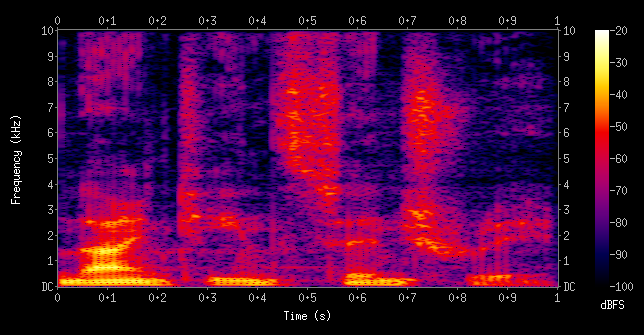
\includegraphics[width=\textwidth]{audio_spectr.png}
    \caption{Пример аудио спектрограммы спокойного произношения слов
    "nineteenth century"\,(перевод на рус. "девятнадцатый век").}
    \label{fig:audio_spectr}
\end{figure}


\paragraph{Компьютерное зрение}
Другим и крайне важным приложением нейронных сетей является
компьютерное зрение. Две наиболее важные использующиеся технологии это
машинное обучение, а конкретно, глубокое обучение и сверточная
нейронная сеть, которая помогает модели машинного обучения
"вглядываться", разбивая изображения на пиксели и присваивая им метки.
Подобно тому как это делает человек, нейронная сеть сначала различает
четкие края и простые формы, а затем заполняет информацию по мере
выполнения итераций своих прогнозов. Сверточная нейронная сеть
используется для обработки отдельных изображений, в то время как
рекуррентная нейронная сеть аналогичным образом используется в
обработке нескольких кадров связанные друг с другом. На рис.
\ref{fig:comp_vision}
приведен снимок того, как нейронная сеть распознает дорогу.
Последовательно применяя к текущему кадру разные фильтры, она пытается
выделить предмет, разбить его на пиксели и обработать эти данные на
основе пройденного обучения.

\begin{figure}[!htb]
    \centering
    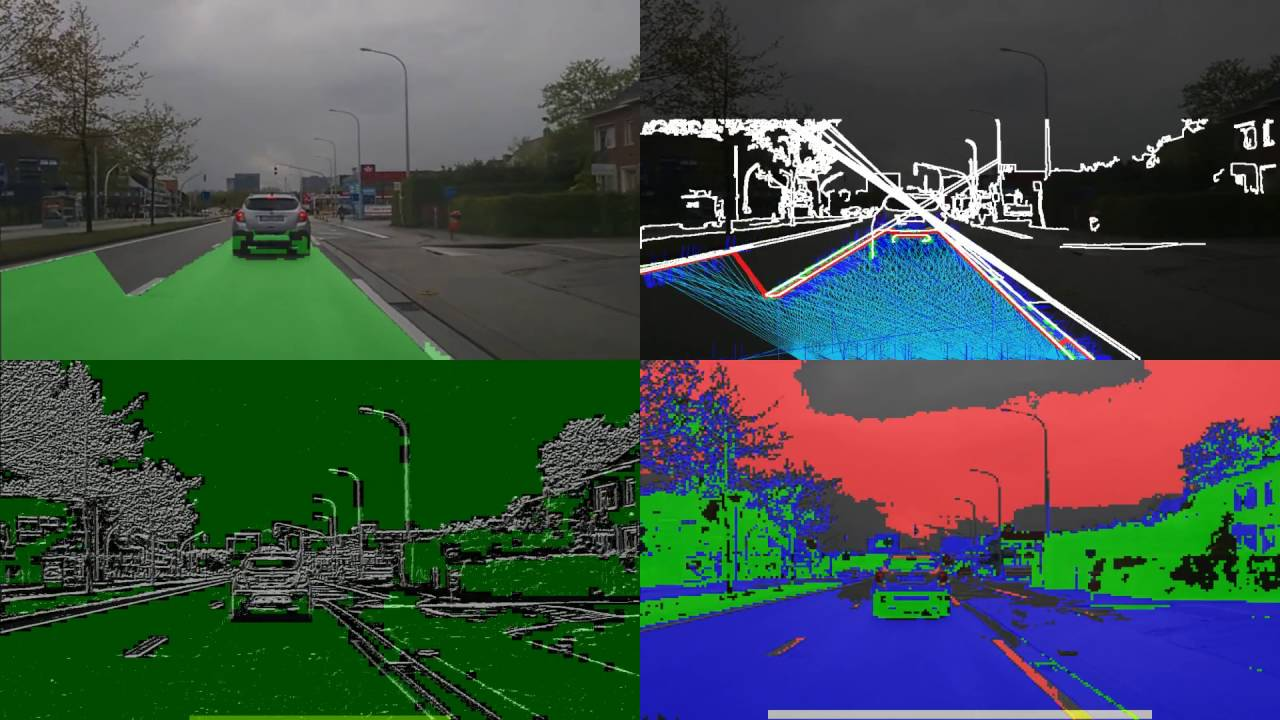
\includegraphics[width=\textwidth]{comp_vision.jpg}
    \caption{Пример распознавания дороги с помощью компьютерного
    зрения}
    \label{fig:comp_vision}
\end{figure}

\chapter{Самоорганизующиеся карты Кохонена}
\chapter{Реализация}

\chapter{Заключение}
\chapter{Приложение}

\end{document}
